% Template file for ICEAA13
%
\RequirePackage{ifpdf}
\documentclass{article}
\usepackage{multirow}
\usepackage{graphicx}

\newcommand{\kvec}{{\bf k}}
\newcommand{\bvec}{{\bf b}}
\newcommand{\shat}{{\hat s}}
\newcommand{\kpr}{{k_\perp}}
\newcommand{\kvpr}{{\kvec_\perp}}
\newcommand{\kpar}{{k_\parallel}}
\newcommand{\AI}{{\langle\tilde A*\tilde I\rangle}}
\newcommand{\AItau}{{\AI(\tau)}}
\newcommand{\hMpci}{{h~{\rm Mpc}^{-1}}}
\newcommand{\inch}{$^{\prime\prime}$}
\newcommand{\foot}{$^{\prime}$}
\renewcommand{\deg}{^\circ}

% In order to produce the pdf document for paper submission either:
% a) process with pdfLaTeX, or
% b) process with LaTeX, dvips, ps2pdf
% In both cases comment out the document class option as indicated above

\newcommand\aj{AJ}%
          % Astronomical Journal
\newcommand\actaa{\ref@jnl{Acta Astron.}}%
  % Acta Astronomica
\newcommand\araa{\ref@jnl{ARA\&A}}%
          % Annual Review of Astron and Astrophys
\newcommand\apj{ApJ}%
          % Astrophysical Journal
\newcommand\apjl{\ref@jnl{ApJ}}%
          % Astrophysical Journal, Letters
\newcommand\apjs{\ref@jnl{ApJS}}%
          % Astrophysical Journal, Supplement
\newcommand\ao{\ref@jnl{Appl.~Opt.}}%
          % Applied Optics
\newcommand\apss{\ref@jnl{Ap\&SS}}%
          % Astrophysics and Space Science
\newcommand\aap{\ref@jnl{A\&A}}%
          % Astronomy and Astrophysics
\newcommand\aapr{\ref@jnl{A\&A~Rev.}}%
          % Astronomy and Astrophysics Reviews
\newcommand\aaps{\ref@jnl{A\&AS}}%
          % Astronomy and Astrophysics, Supplement
\newcommand\icarus{\ref@jnl{Icarus}}%
  % Icarus
\newcommand\mnras{\ref@jnl{MNRAS}}%
          % Monthly Notices of the RAS
\newcommand\prc{\ref@jnl{Phys.~Rev.~C}}%
          % Physical Review C
\newcommand\prd{\ref@jnl{Phys.~Rev.~D}}%
          % Physical Review D
\newcommand\pre{\ref@jnl{Phys.~Rev.~E}}%
          % Physical Review E
\newcommand\prl{\ref@jnl{Phys.~Rev.~Lett.}}%
          % Physical Review Letters
\newcommand\pasa{\ref@jnl{PASA}}%
  % Publications of the Astron. Soc. of Australia
\newcommand\pasp{\ref@jnl{PASP}}%
          % Publications of the ASP


\title{The Hydrogen Epoch of Reionization Array (HERA)}

% Use \thanks{} for each affiliation.
% If the authors have the same affiliation, use \thanks[n] to
% refer to the same affiliation of the n:th \thanks command
\author{A.U. Thor\thanks{Institution}
}
\begin{document}
\maketitle


\section{Abstract}
\label{sec:abstract}
The Hydrogen Epoch of Reionization Array (HERA http://reionization.org) is a staged experiment that uses the unique properties of the 21-cm line from neutral hydrogen to probe the Epoch of Reionization (EOR). During this epoch, roughly 0.3 - 1 billion years after the Big Bang, the first galaxies and black holes heated and reionized the early Universe. Direct observation of the large scale structure of reionization and its evolution with time will have a profound impact on our understanding of the birth of the first galaxies and black holes, their influence on the intergalactic medium (IGM), and cosmology.  This paper will provide an overview of the project and describe the design of the system.

\section{Introduction}
\label{sec:intro}
We have garnered a deep understanding of the large scale structure of the very early Universe by observing the faint afterglow of the cosmic microwave background (CMB).  The CMB signal arises due to the recombination of hydrogen gas which allows the radiation to stream forth.  It represents one slice in time when the faint imprint of the nearly homogeneous inflationary Universe may be seen.

We also have a good understanding of the complicated structure and denizens of our current Universe.  In between however, we have very little information of how our Universe evolved to its current structure.  It is as if we have one detailed snapshot from one day in the first days of our baby's life, and then a Facebook page of our child as a young adult with very little in between except faint rumors and a headline or two.

This intervening period has essentially four phases which may be called the Dark Ages, the Cosmic Dawn, the Epoch of Reionization (EOR) and the Rise of the Galaxies.  The time of the Cosmic Dawn saw the first large-scale gravitational collapse of structures, which eventually heated up the neutral intergalactic hydrogen gas until it again ionized.  This phase change is called the Epoch of Reionization and it represents the last phase change of the Universe as a body.  We may observe this epoch over its extent by observing the red-shifted hydrogen gas.  In our analogy, this is akin to following our child's activities and growth through a good part of their formative years.  Fig. \ref{fig:cosmos} shows a depiction of the history of the Universe, as well as the 21-cm Hydrogen line red-shifted to cosmic time.

\begin{figure}[t]
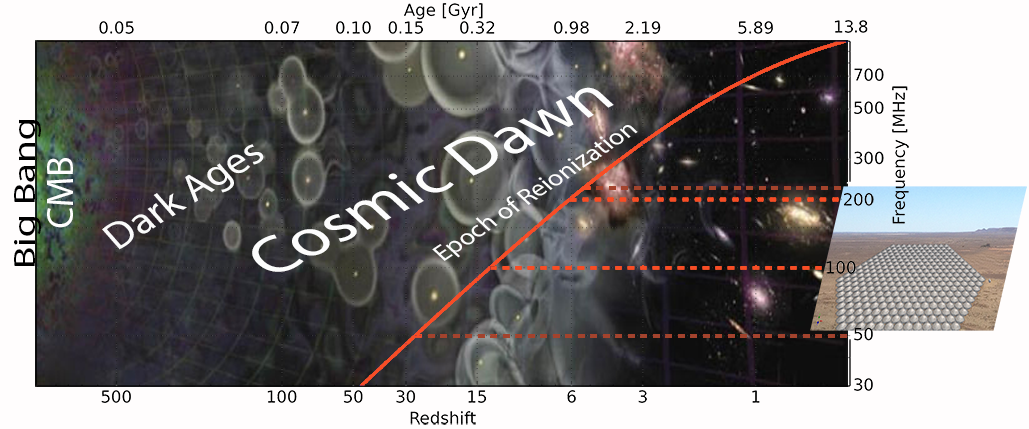
\includegraphics[width=\textwidth]{plots/herauni/herauniall.png}
\caption{history of the Universe plotted on a log scale.  The top axis shows the time elapsed since the Big Bang while the bottom shows the corresponding redshift.  Of course, placing exactly when the depicted events occurred and how is the goal of HERA.  The right axis and the red-line show the frequency of the 121-cm Hydrogen line over cosmic time.  The horizontal lines denote the frequency range of HERA, both the initial band (the inner pair) and the desired extended band.  CREDIT BACKGROUND IMAGE - GET PERMISSION
\label{fig:cosmos}}
\end{figure}

Detecting, characterizing and ultimately imaging the Epoch of Reionization is a key goal for the astronomy and astrophysics community. There are many references on the theoretical, instrumental and observational foundations, see for example one of the latest instrument papers and references therein ({\em e.g.} {\cite{2015arXiv150206016A}}).  Current projects (PAPER (http://eor.berkeley.edu), MWA (http://mwatelescope.org), LOFAR (http://www.lofar.org)) are striving to make the first detection of the statistical power spectrum of the signal, however current best limits still fall above even optimistic predictions of its intrinsic strength.  While these projects are still taking data, it is recognized that an optimized array based on our new understanding of the signal characteristics is needed to make a strong detection and begin to characterize this signal over multiple scales and redshifts.  These results would also inform design elements for the Square Kilometer Array (http://www.skatelescope.org).

The Hydrogen Epoch of Reionization Array (HERA http://reionization.org) is a staged experiment that uses the unique properties of the 21-cm line from neutral hydrogen to probe the EOR, roughly 0.3 - 1 billion years after the Big Bang. Direct observation of the large scale structure of reionization and its evolution with time will have a profound impact on our understanding of the birth of the first galaxies and black holes, their influence on the intergalactic medium (IGM), and cosmology.

\begin{figure}[t]
\includegraphics[width=0.45\textwidth]{plots/HERA_array.png}
\includegraphics[width=0.45\textwidth]{plots/IMG_3538.png}
\caption{Perspective cartoon of the 331-element core within a 305-meter circle.  With current picture.
\label{fig:array}}
\end{figure}

HERA has been funded under the US National Science Foundation's Mid-Scale Innovations Program to begin building elements optimized for robust power spectrum detection.  The key is to produce inexpensive collecting area optimized to detect the EOR.  This has resulted in a close-packed array of transit 14-meter dishes (Fig. \ref{fig:array}), with the first elements currently under construction at the South African Karoo Astronomy Reserve, the current location of the Donald C. Backer Precision Array to Probe the Epoch of Reionization (PAPER) array.  [PAPER REF]

Beginning with the current NSF funding, HERA is rolling out in a staged deployment.  The first phase extending to August 2016 will deploy 37 elements that will test the HERA element design for performance and manufacturability at location.  These 37 elements will more than double the sensitivity of the 128-element PAPER array.  The next phase extending into 2018 will build out to 127 elements, which should provide a very robust detection of the EOR signal.  Finally, extending into 2020, HERA will build out to 352 elements to further EOR science as a function of redshift and spatial scale, potentially producing the first images of the EOR.

HERA is a collaboration of the following partner institutions:  Arizona State University, Brown University, University of California Berkeley, University of California Los Angeles, University of Cambridge, Massachusetts Institute of Technology, National Radio Astronomy Observatory, University of Pennsylvania, SKA-South Africa, and
University of Washington.

\section{Measuring the EOR}
\label{sec:eormeas}
Due to the expansion of the Universe, we can identify and measure the early Universe via the red-shift of spectral lines.  The hydrogen hyperfine transition at a rest frequency of 1420 MHz is a key spectral line due to the ubiquity of hydrogen and, being a ``forbidden'' transition, the optical depth lets us see through the entire Universe back almost to the period of recombination.  The bandwidth
therefore equates to a cosmic volume along the site of the telescope, with the frequency determining the cosmic age.

Given the difficulty of the experiment, initial measurements of the EOR strive to measure a statistical power spectrum of the signal since the nature of the reionization process should have a specific spatial signature.  The goal is therefore to measure a range of aggregate spatial scales on the sky, rather than to image the signal directly.  Imaging does remain an ultimate goal to fully understand the process, however we will need a greater understanding of the full measurements to achieve this more difficult goal.  

Obviously between our present observation point and the Epoch of Reionization approximately 13 billion years ago lies the entire intervening Universe, which has an intrinsically much brighter signal (up to 6 orders of magnitude or more).  Primarily, this power is due to diffuse Galactic synchrotron radiation, supernova remnants and extragalactic radio sources.  As a first step, areas of the sky with where these signals are minimal (for example, outside the galactic plane and away from strong point sources) are targeted (REF FOR THIS).  More importantly and most fortuitously however is the fact that all of these signals are smooth spectrum sources whereas the expected spectrum of the EOR is expected to be rough since it is made up of non-ionized regions which are randomly distributed over a wide range of redshifts.  This fact allows us to try and isolate foregrounds from the EOR, as will be discussed.

Though the desired measurement is over a volume, it is instructive to split it into two components,  $\kvec =  \kvpr + \kpar{\hat {\bf z}}$ where $\kpr$ is determined by the antenna baseline and $\kpar$ by the frequency.  This is useful since it allows us to split out the chromatic response of the interferometer and isolate a phase space where foreground sources ({\em i.e.} everything not the EOR) contaminate the signal of interest from where they don't.  This contaminated phase space may be shown [REF] to be a wedge-shaped region in $\kpr$:$\kpar$ space:
\begin{equation}
|\kpar| \le \beta\frac{X\lambda}{Yc}\kpr + \frac{S}{Y}
\end{equation}
where $c$ is the speed of light and $S$ is a parameter accounting for offsets related to the combined spectral smoothness of the foregrounds and the antenna response (see Fig. \ref{fig:wedge}).  
A key issue to measuring the EOR power spectrum is to understand and minimize such effects.  For an analytical derivation, see \cite{2012ApJ...756..165P,vedantham_et_al2012,liu_et_al2014b},  in simulation see \cite{datta_et_al2010,hazelton_et_al2013} and for observations
\cite{2013ApJ...768L..36P,2015arXiv150601026P,2014ApJ...788..106P,2015arXiv150206016A}.

\begin{figure}[t]
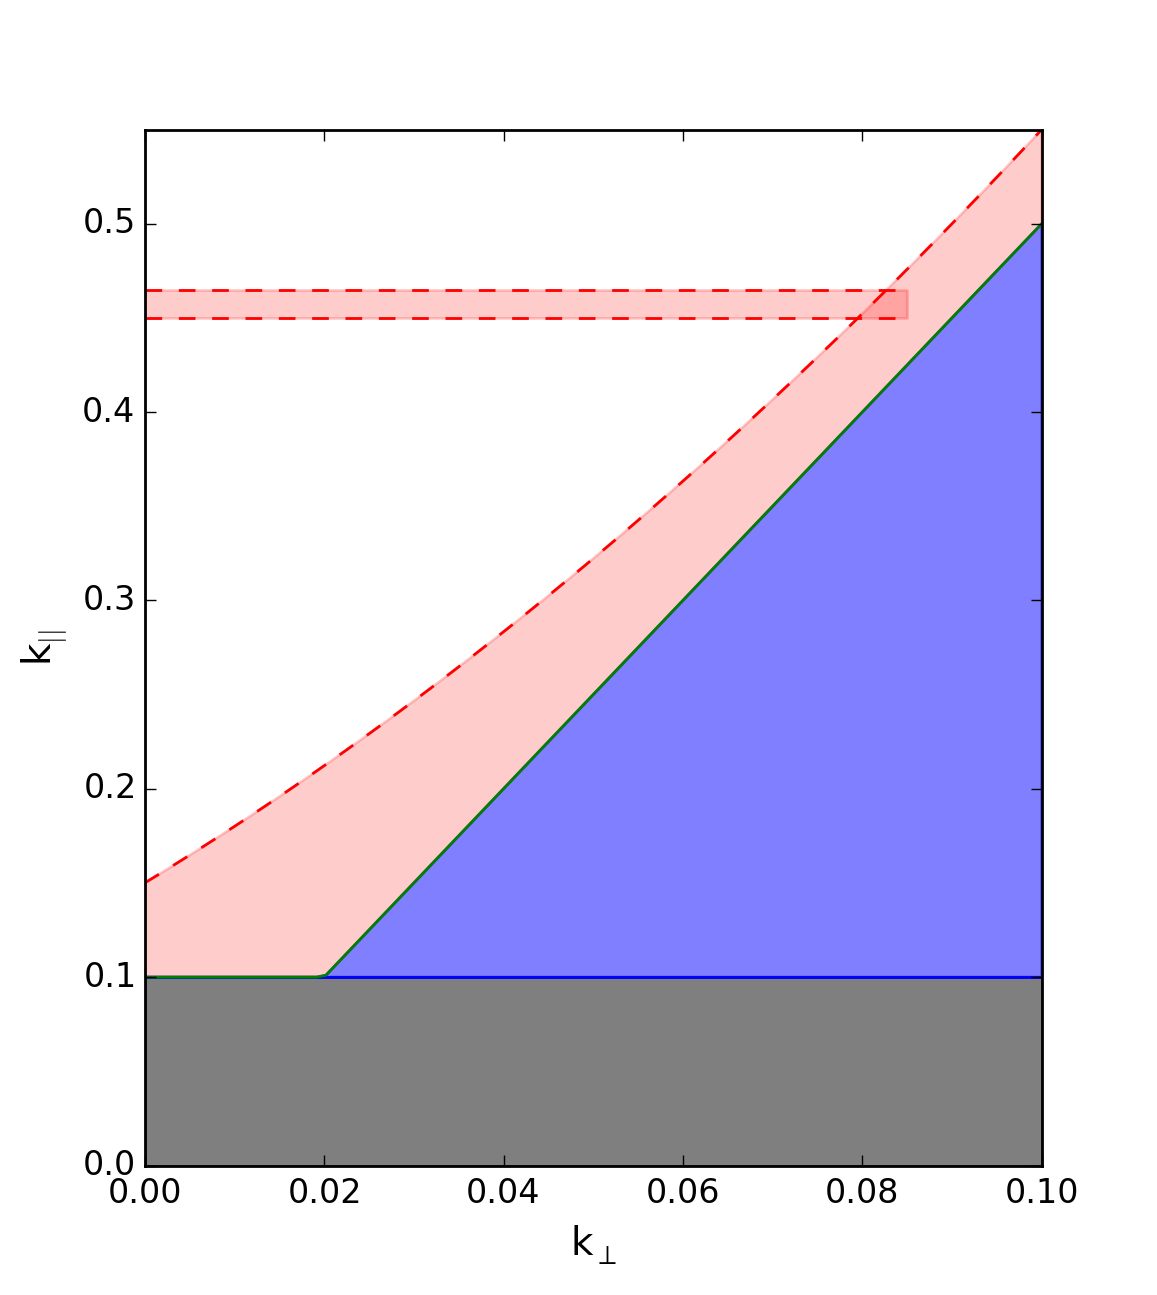
\includegraphics[height=3in]{plots/wedge.png}
\caption{Cartoon of the wedge.  The gray rectangle represents the smooth-spectrum foregrounds as they would be if the instrument had a perfect achromatic response.  The pink wedge area shows the chromatic response of the interferometer, where additional power is thrown up from the gray region to higher k-values with increasing baseline.  The additional horizontal pink line illustrates the affect that other systematics, such as reflections on cables, can have in contaminating the measurement.  The white region shown the 'eor window', where the measurement is not contaminated by foregrounds or systematics.
\label{fig:wedge}}
\end{figure}

The techniques to measure the power spectrum may be broken down into two principle techniques, plus additional hydrid methods.  These are briefly summarized below.

\subsection{Delay-Spectrum Approach}
\label{sec:delayapproach}
Given that the response of an interferometer natively measures the power in Fourier modes of the sky within its beam, we see that it is a natural instrument to use for this measurement.  There are now numerous papers in the literature the technique of measuring the power spectrum using an interferometer and the attendant issues (list of citations).  Below, a high-level overview based on  \cite{2012ApJ...756..165P} will be presented. The so-called delay-spectrum approach leverages this response to optimize sensitivity to the desired modes while rejecting modes contaminated by the foreground power in the wedge.  Other than potentially handling overlapping bins in {\em uv} space, the delay-spectrum approach does not combine baselines before squaring and calculating the power spectrum.

We can essentially relate the sky power spectrum mode ${\hat P}(\kvec)$ to an interferometer baseline visibility ${\tilde V}(\bvec)$, which is the equivalent of the (complex) fringe pattern in a double slit experiment:
\begin{equation}
{\hat P}(\kvec) \approx\frac{X^2Y}{4k_B^2}   \left[\frac{{\tilde V}^2(\bvec)}{\Omega_b B/ \lambda^4} \right]
\label{eq:Pk_baseline}
\end{equation}
where $X$ and $Y$ are cosmological parameters relating angular size and spectral frequency to cosmic volumes, $\Omega_b$ is the integrated beam response, $B$ is the effective bandwidth, $\lambda$ is the observation wavelength, and $k_B$ is Boltzmann's constant.  The terms in square brackets are instrumental terms, as opposed to the constants and cosmological parameters.  Rather than ${\hat P}(\kvec)$, the literature generally works with a volume-normalized parameter given by $\Delta^2(k) = \frac{k^3}{2\pi^2}{\hat P}(\kvec)$.

Since the thermal noise per visibility baseline may be expressed as
\begin{equation}
V_N = \left(\frac{2k_B}{\lambda^2}\right)\left(\frac{T_{sys}}{\sqrt{2B\tau}}\right)\Omega_b B
\label{eq:sensitivity_per_baseline}
\end{equation}
where $\tau$ is the integration time (see {\em e.g.} TMS),
to determine the sensitivity of an instrument to the power spectrum per baseline we can substitute the thermal noise per baseline for the visibility in Eq. \ref{eq:Pk_baseline}.  Further, since an interferometer typically measures many baselines which may be averaged together to improve the signal-to-noise per $k$-bin, the total sensitivity may be approximated as
\begin{equation}
\Delta^2_N (k,z)\approx \frac{k^3X^2(z)Y(z)}{4\pi^2} \left[\frac{T_{sys}^2(z)\Omega_b(z) }{\tau(z) \mathcal{N}_s(k)}\right]
\end{equation}
where $\mathcal{N}$ represents the improvement in sensitivity for coherently and incoherently averaging $k$-bins, depending on the configuration and technique (see \ref{parsons12b}).

The power spectrum uses the full magnitude of the {\bf k}-vector, which is set by the antenna baselines and bandwidths.  Note that largest bandwidth (which determines the smallest $\kpar$) is about 10 MHz, for larger bandwidths cosmic evolution begins to impact the result.  Figure \ref{fig:kperf} shows the allowed k-values based on the beamwidth/baseline (gray plus dark-blue overlap regions, the black lines are the limits) and a bandwidth of 10 MHz with 1024 channels (the blue and dark-blue overlap regions, the blue line is the lower limit).  The red-dashed line is the allowed smallest k-value that can be measured.  Note that at these red-shifts it is essentially set just by the bandwidth.

\begin{figure}[t]
\centerline{
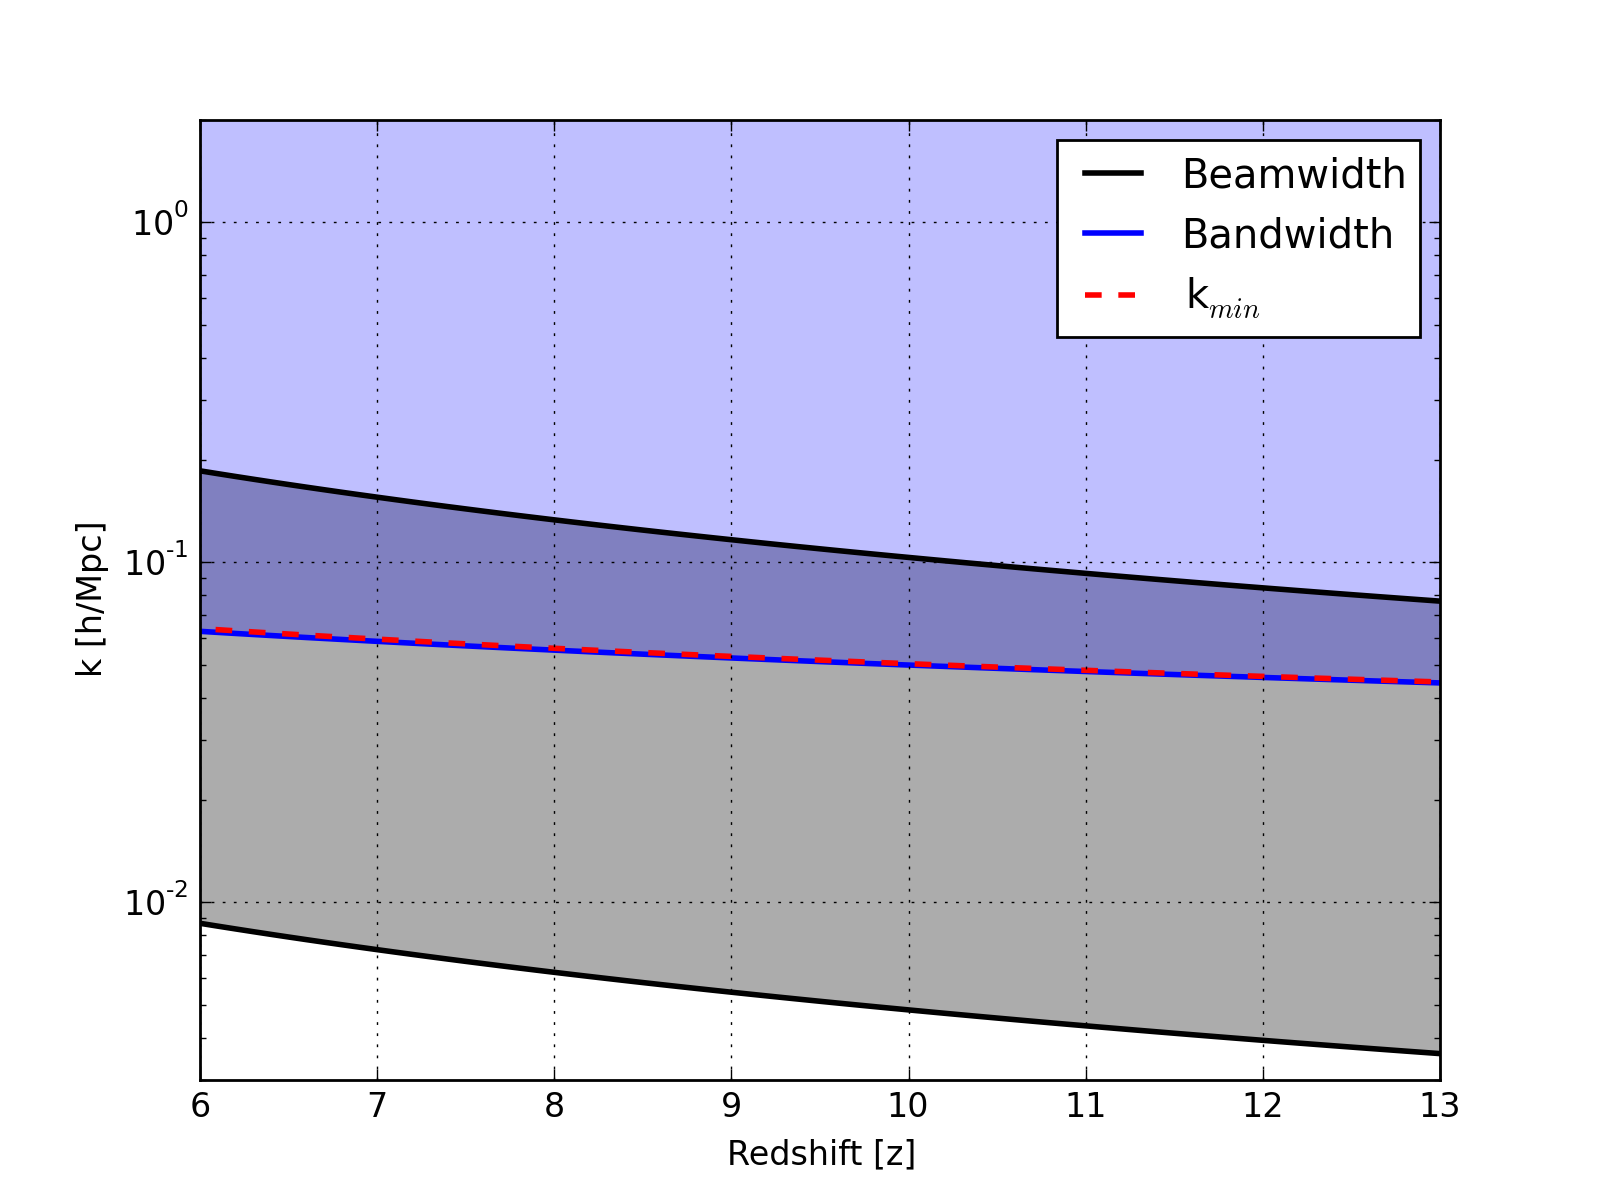
\includegraphics[width=\textwidth]{plots/kperf_heraZ.png} 
}
\caption{\small k
\label{fig:kperf}}
\end{figure}

\subsection{Map-Making Approach}
\label{sec:mapapproach}
In contrast to the delay-spectrum approach, map-making approaches combine baselines to build up information before squaring and calculating the power spectrum.  The conceptually easiest approach is that one makes an image of the sky and takes a 2-D Fourier transform to determine the power spectrum.  Advantages are that you actually image the reionized bubbles and can determine the magnitude of the smaller k-modes on the sky.  The principle disadvantage is that you have to compute and calibrate the effects of systematics and the propagation of the very bright foregrounds through your system and subtract them incredibly accurately.  In contrast, the delay-spectrum approach localizes those effects to a parameter space where they can much more easily be filtered and not used in subsequent analysis.

\subsection{Hybrid Approaches}
\label{sec:hybridapproach}

\section{Scientific Requirements and Specifications}
\label{sec:specs}
As the initial detection and analysis approach is primarily focused on the delay-spectrum approach, the requirements are set primarily by that approach.  However, since the map-making approaches remain a goal, the design makes every effort to allow such studies.  The high-level specifications are summarized in Fig. \ref{fig:array}.  Specifications fall within one of three categories:  Phase 1, Phase 2, or Extended.   

\begin{enumerate}
\item {\em Phase 1} corresponds to the current stage where the existing analog and digital signal chains are used with the new HERA element.  Ostensibly, this corresponds to the first two years where the total number of HERA elements remains less than 128.  This allows for a strong transition period with a known signal path but with new elements.
\item {\em Phase 2} corresponds to the upgraded signal path slated for when the element count exceeds 128 and the architecture changes to allow extensibility and improved performance.
\item {\em Extended} are those goals that are aspirational on a best efforts basis, or that include additional science beyond the EOR.
\end{enumerate}

\begin{table}
\label{tab:specs}
\caption{Overview of requirements and specifications}
\begin{tabular}{| l | l | l | p{5cm} |}\hline
{\bf Parameter} & {\bf Requirement} & {\bf Value} & {\bf Comments} \\ \hline
Frequency range & 100 - 200 MHz & & Phase 1 \\ \hline
Number of channels & $>$256 & 1024 & \\ \hline
Diameter    & $<$ 14.1 m &  14.0 m & Picked near requirement for sensitivity/cost \\ \hline
Shortest baseline & $<$ 15 m & 14.6 m & \\ \hline
\end{tabular}
\end{table}

\subsection{Spectral Response:  Frequency Range and Bandwidths}
Figure \ref{fig:cosmos} highlights the frequency range requirement to probe the expected timescale of the epoch of reionization using the 21cm line of hydrogen as the probe.  
These limits are derived from to-date complementary probes of reionization which include measurements of
the optical depth to last scattering in the CMB, QSO spectra, Ly-$\alpha$
absorption in the spectra of quasars and gamma ray bursts and the demographics
of Ly-$\alpha$ emitting galaxies
%We show limits established by some of these techniques in
(Figure~\ref{fig:IonHist}). 
Constraints from these probes are still weak:
Ly-$\alpha$ absorption saturates at very small neutral fractions; galaxy
surveys directly constrain only the bright end of the luminosity function and
depend on an unknown escape fraction of ionizing photons to constrain
reionization; CMB measurements probe an integral quantity subject
to large degeneracies. Even when these observations are
combined into a single 95\% confidence region, the bounds remain weak.
For example, $x_{HI}$ spans almost the entire allowable range of [0,1]
at $z=8$. 21\,cm reionization experiments place much tighter constraints on ionization, with the
red band showing the forecasted 95\% confidence region derived from HERA data,
after marginalizing over astrophysical and cosmological parameters.

****Include references

From these measurements and models, the Phase 1 and 2 minimum spans of redshifts range from $z=$6 to 13, corresponding to a frequency range of 100 - 200 MHz.  Extending the science to include the Dark Ages remains a goal so that efforts are on-going to design a feed to increase the lower limit down to about 50 MHz without compromising the performance in the specification range.  The fall-back position for the low-frequencies is a serial deployment of a scaled version of the HERA feed or to potentially build additional elements specifically for the low-frequencies.  The 100 MHz bandwidth is also the minimum fully digitized and correlated bandwidth.

The scientific requirement on channel bandwidth is to allow access to k-modes of greater than 1 h/Mpc [ref], which requires about 256 channels over the 100 MHz bandwidth.  However, in order to handle radio frequency interference as well as to allow the bandpass to be characterized, a specification of 1024 channels has been chosen.  This yields a channel bandwidth of 97.7 kHz.


\subsection{Spatial/Delay Response:  Diameter and Minimum Baseline}
The spatial response provides the defining characteristics for the experiment; related to the diameter, focal length, baseline, and configuration.  The principal constraint sets the delay response of the antenna element, characterized by the magnitude and frequency of the antenna ripple response.  This was initially addressed to first order in [MEMO] and in a much more detailed way in [UPCOMING PAPERS].  Expressed simply, the delay response of the antenna must be sufficiently attenuated such that the foreground signal levels at those delays is below the expected signal strength of the EOR signal.  This sets the optics and match needs.  As discussed in [REFS], this is addressed by direct measurement and modeling of the response to the system relative to and as a function of delay time from the initial wave reception.  The expected strength of the foregrounds is modeled through the system and plotted on the same set of axes.  These two regions should be disjoint to a significance of 60 dB.

In order to do an initial design and a parametric study, the approach used first sets a specification on the magnitude of the feed/vertex reflections within the dish for 1, 2, and 3 round-trip travel delay times.  Reference \cite{heraMemo5} provides an initial estimate that the reflections must be down by 60 dB on timescales greater then 60 nanoseconds.  
Also in ref \cite{heraMemo5}, an analysis using a feed pattern based on the existing PAPER dipole antenna with a fairly complete analytical model of a prime focus antenna, the effective area was found to be maximized for $f/D \approx 0.32$.  Figure \ref{fig:costfig} shows the vertex/feed round-trip travel times for one, two and three reflections.  

Interpreting Fig \ref{fig:costfig} is somewhat confusing, but note that the vertical color scale represents a fairly steep cost function preferring delay time-scales of less than 60 ns (ignoring the horizontal color scale for now, to be discussed in Sec \ref{sec:cost}).  The preliminary study requirement is to ensure that reflections are down by about 60 dB by that time-scale.  As seen by the black dashed line labelled '1' for one round-trip between the feed and vertex, for the focal ratio and diameters of interest  this reflection is always less than 60 ns, so this does not constrain the design.  For two round-trips (black solid line labelled '2'), we see that for diameters greater than 14.1m, the delay is less than 60 ns, so diameters less than this are preferred.  For three round-trips, we see that we would need antennas with diameters smaller than 9.4m.  However, cost (sec. \ref{sec:cost} and practicality issues ({\em i.e.}physically moving within the filled array) make these small diameters undesirable, so this means that we need to ensure that our system has sufficiently damped reflections for 3 reflections.  This is discussed in detail in UPCOMING PAPERS.  We have therefore adopted a specification that the antenna must be less than 14.1 meters in diameter.

The minimum baseline is set such that the baseline has negligible impact on the minimum $k_{bin}$ (shown in Fig. \ref{fig:kperf}) in the standard analysis.  Somewhat arbitrarily, a maximum shortest baseline with equal contribution to $k_{min}$ at the full bandwidth of 100 MHz is chosen, which corresponds to about 15m.  Additionally, this baseline has been well-studied by the PAPER array (ref) and is consistent with the diameter specification derived above.

\begin{figure}[t]
\centerline{
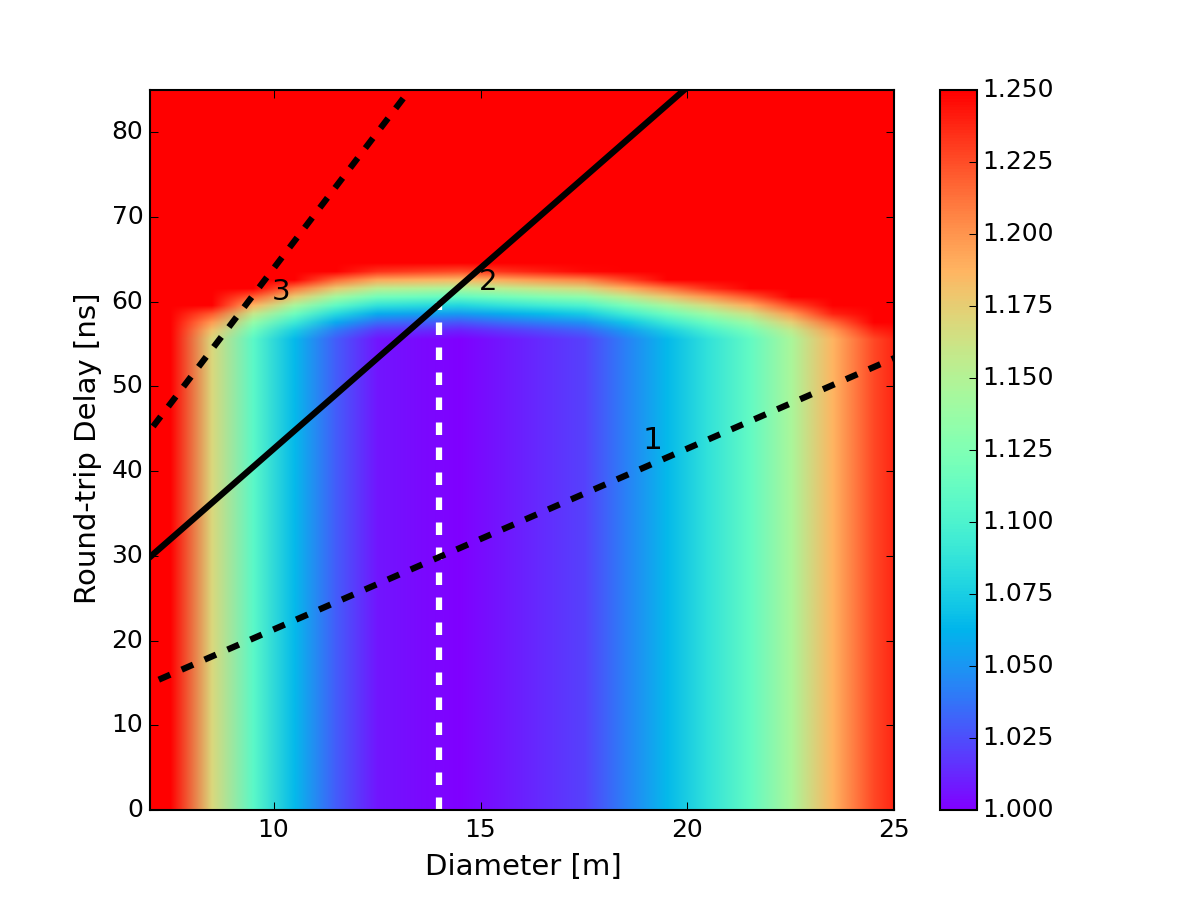
\includegraphics[width=7.5cm]{plots/costfigNew.png} 
}
\caption{\small Costing model for a fixed sensitivity system as a function of diameter (thick blue line and left axis) as well as the round-trip delay for 1,2 and 3 feed-vertex trips (dashed red lines and right axis).  The 60 ns spec is indicated by the horizontal dash line, and the two-trip intersection at about 14-meter is the vertical dashed line.  SEE TEXT...
\label{fig:costfig}}
\end{figure}

\subsection{Sensitivity:  Diameter, Number, and Configuration}
What is our requirement?

sensitivity - reionization fraction 10$\sigma$ from 0.2-0.8?

10\% estimate of neutral fraction?

\begin{figure}[t]
\centerline{
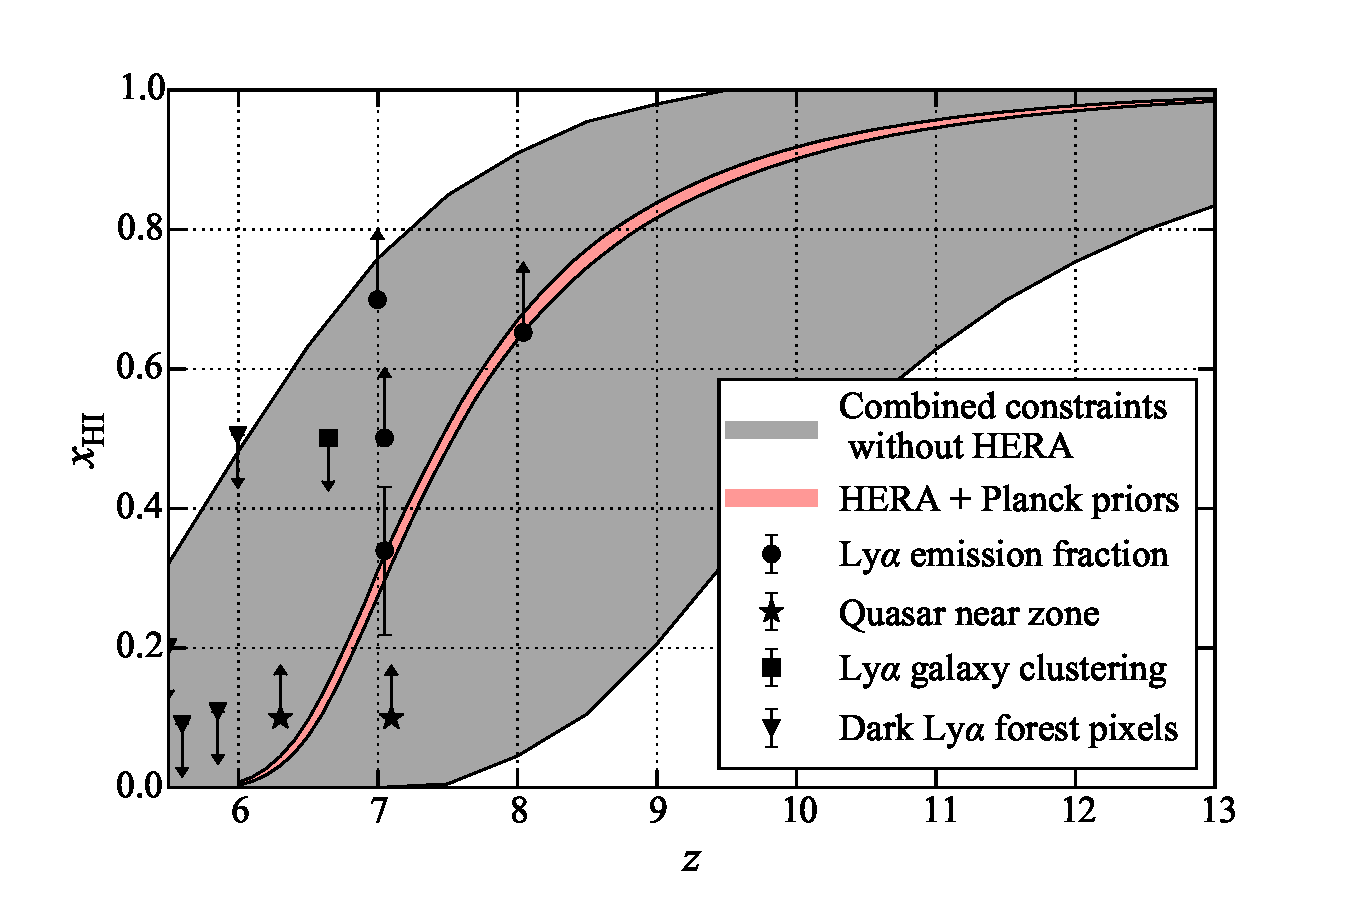
\includegraphics[width=.3\textwidth]{plots/ionHist.pdf}
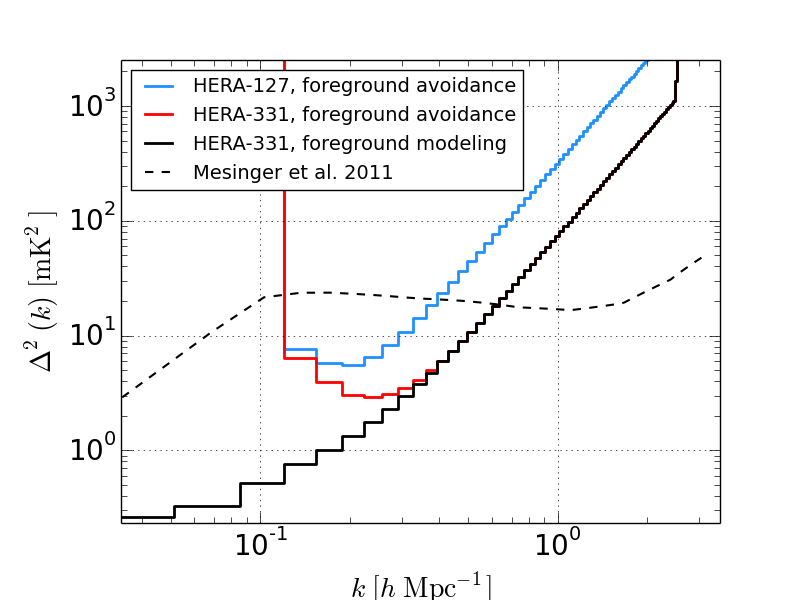
\includegraphics[width=.3\textwidth]{plots/eor_pspec_2014.png}
\includegraphics[width=.3\textwidth]{plots/HERA_sensitivity.pdf}
}
\caption{\small Sensitivity
\label{fig:sensivity}}
\end{figure}

\subsection{Cost}
\label{sec:cost}




\section{HERA System Overview}
\label{sec:system}
STAGED APPROACH WITH PAPER FIRST

HERA will operate between 70 MHz and 220 MHz, however the first phases (up to 127 elements) will operate within the current PAPER bandwidth of 110-190 MHz.  The full band is directly sampled and correlated, making for a very simple signal path requiring only gain.  Initially, the exact PAPER signal chain will be used, which brings the RF back to a central container on coaxial cable where it is digitized and processed.  A new modular digitizer (Smart Network ADC Processor, or SNAP) has been developed that will be deployed in the field and will shorten the amount of RF cable.  The digitized signal will be conveyed back to a central building for processing via 10 Gbit ethernet over fiber-optic cable.   The SNAP board is being developed as part of the CASPER suite of hardware components (https://casper.berkeley.edu/wiki/DAB-HERALD).  A simple block diagram of the two-phase system is shown in Fig. \ref{fig:system}.

\begin{figure}[t]
\centerline{
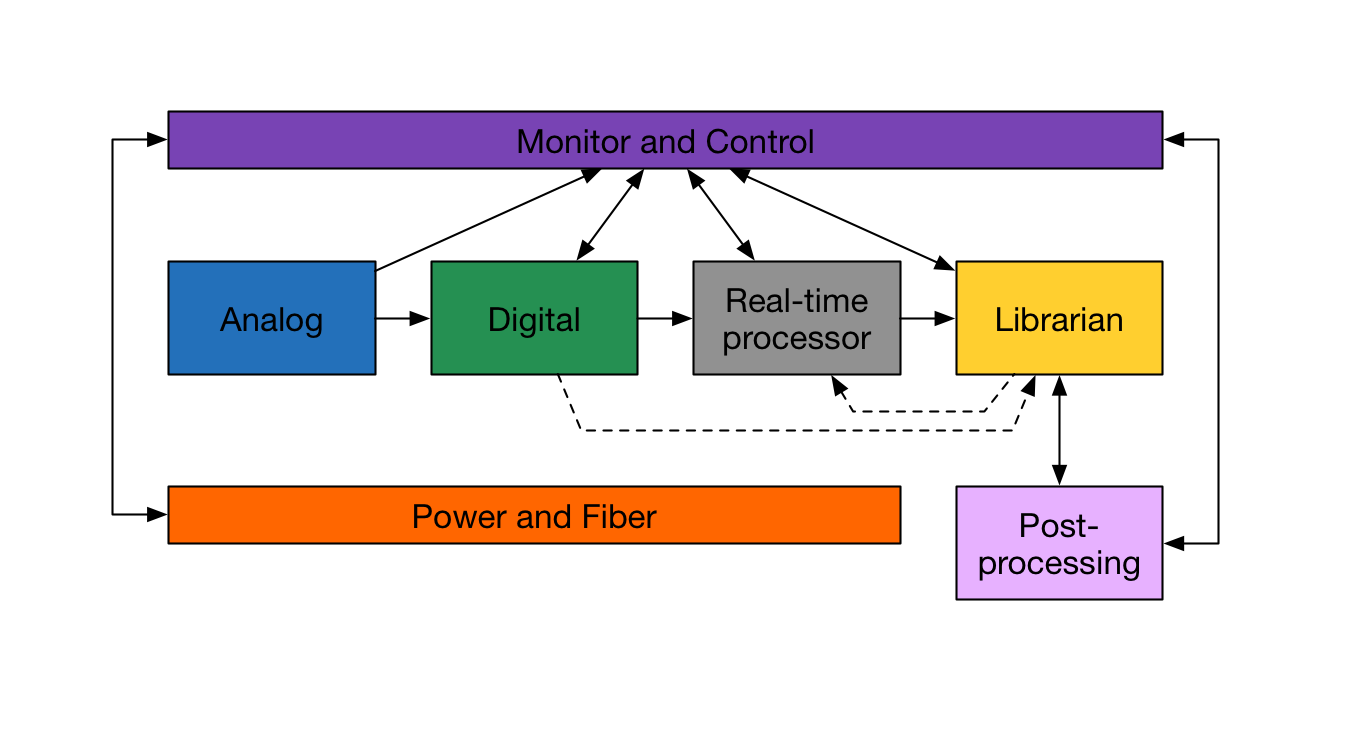
\includegraphics[width=\textwidth]{plots/sysOver.png} }
\caption{\small Architecture of HERA.
\label{fig:architecture}}
\end{figure}

\begin{figure}[t]
\centerline{
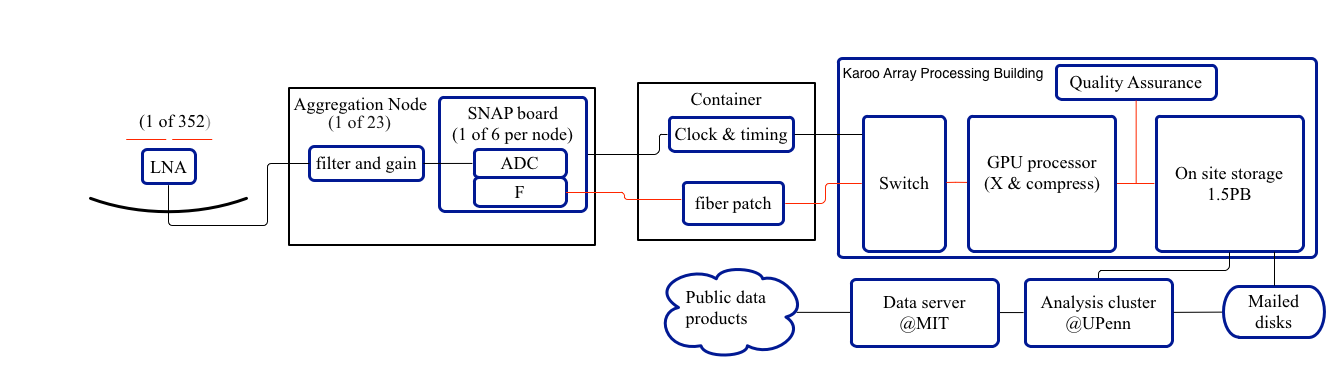
\includegraphics[width=\textwidth]{plots/HERA_high_level_block_diagram.png} }
\caption{\small High-level block diagram of the HERA system.  The dashed lines indicate the first phase while solid are the final design.  Black lines are coaxial cable and orange are ethernet over fiber.
\label{fig:system}}
\end{figure}

The configuration is optimized for power spectrum detections, which favors as large of a fill-factor as possible.  The configuration is therefore a packed hexagonal array with a 14.6-meter pitch with a 14-meter antenna (see Fig \ref{fig:config}).  Additionally, there will be 21 outriggers out to 1.2km to improve the resolution 

%\begin{table}[htpb]
%\centerline{
%\begin{tabular}{|l||c|c||c|c||}\hline
% \multirow{2}{*}{Instrument}                 & \multicolumn{2}{|c|}{Avoidance} & \multicolumn{2}{|c|}{Subtraction} \\ \cline{2-5}
%                      & Drift  & Track  & Drift  & Track \\ \hline
%PAPER 128  &  1.56  &  -  &  4.46  &  - \\ \hline
%MWA 128      &  0.66  & 0.86  &  2.50  &  3.15 \\ \hline
%LOFAR (core) & 0.70  & 1.90  & 7.48  &  12.22 \\ \hline \hline
%HERA 37         & 5.67  &  -  & 15.46   &  - \\ \hline
%HERA 331       & 38.75 & -  &  111.69  &  - \\ \hline
%MWA 256         &2.40   &  2.81  &  8.28  & 9.64 \\ \hline
%SKA1 Low      &21.23   & 26.92  & 139.07  & 115.13 \\ \hline
%\end{tabular}}
%\caption{\small Parameters and their values; units are spaced from the
%corresponding measure by an unbreakable thin space and should
%always be in upright font.\label{tab:sensitivity}}
%\end{table}



\subsection{Element and Analog Signal Path}
\label{sec:element}
The design of the HERA element is discussed in \cite{heraMemo5}.  The design principles are three-fold:
\begin{itemize}
\item optimize for the delay-spectrum technique of measuring the EOR power spectrum,
\item minimize costs, and
\item the experiment has a limited lifetime of about five years.
\end{itemize}
The first item primarily means that chromatic effects corresponding to delays appropriate for the measurement described above must be below the expected signal level, which essentially determines the focal length.  The second item constrains the diameter and element count, as well as the focal length over diameter ratio ($f/D$), based on a cost function and maximizing sensitivity per element.  And the third items constrains the construction materials and methods and the operational model.



To determine the optimal diameter, full system costings were done on a range of diameter sizes from 5m - 25m, where the total number was constrained to keep constant sensitivity for this measurement, which is shown in Figure \ref{fig:costfig}.  By assuming canonical values of 331 14-meter antennas, the number of elements needed for a given diameter to match the sensitivity is
\begin{equation}
N_a = 4634/D_a
\end{equation}
Figure \ref{fig:costfig} shows the resulting normalized system cost/performance-curve, which becomes quite flat for diameters greater than about 14m, which also happens to be the diameter where two reflections between the feed and vertex coincide with the 60 ns specification.  An addition high-level analysis of reflection coefficients within the structure also indicate that a diameter of less than 15 meters is preferred.  The diameter of 14 meters was therefore chosen for the element.

A full-sized prototype of this system was built and measured using a network analyzer in time-domain mode, which meets the ``60 by 60 '' specification (Fig \ref{fig:refl}). (\cite{heraMemo5}).

\begin{figure}[t]
\centerline{
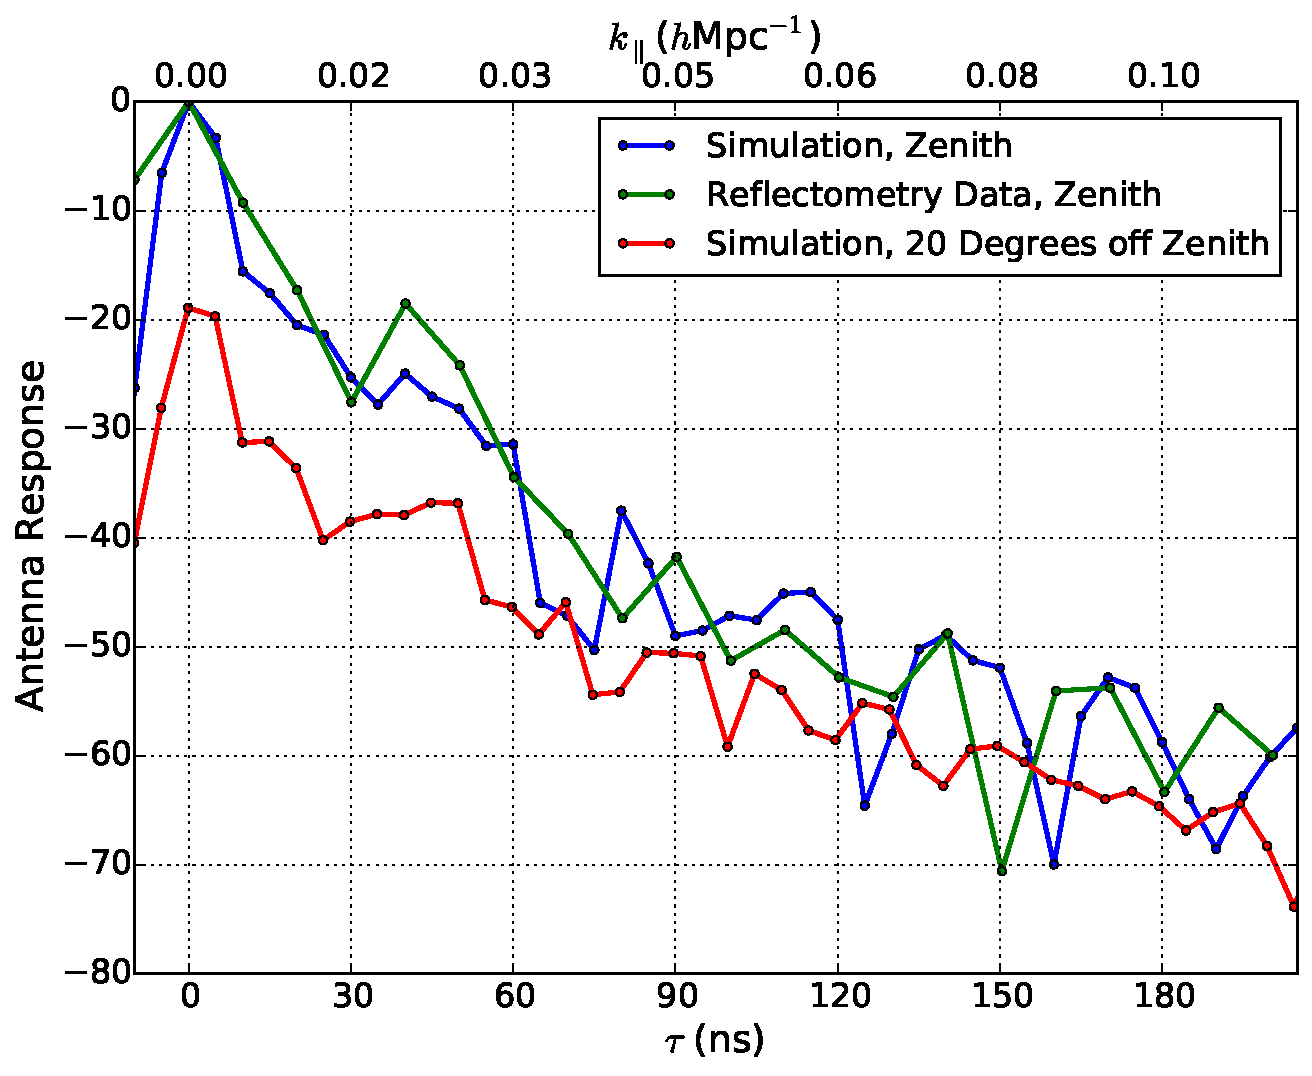
\includegraphics[width=\textwidth]{plots/compareSimToDataNormalized.pdf} 
}
\caption{\small Simulations/measurements of reflected power versus delay time of the full-size HERA prototype.
\label{fig:refl}}
\end{figure}

\subsection{Digital Signal Path}
\label{sec:DSP}

\subsection{Real-Time Processor and Librarian}
\label{sec:rtplib}

\subsection{Monitor and Control}
\label{sec:moncon}

\subsection{Infrastructure}
\label{sec:infra}

\subsection{Post-Processing}
\label{sec:postproc}

\subsection{Configuration}
\label{sec:config}
\begin{figure}[t]
\centerline{
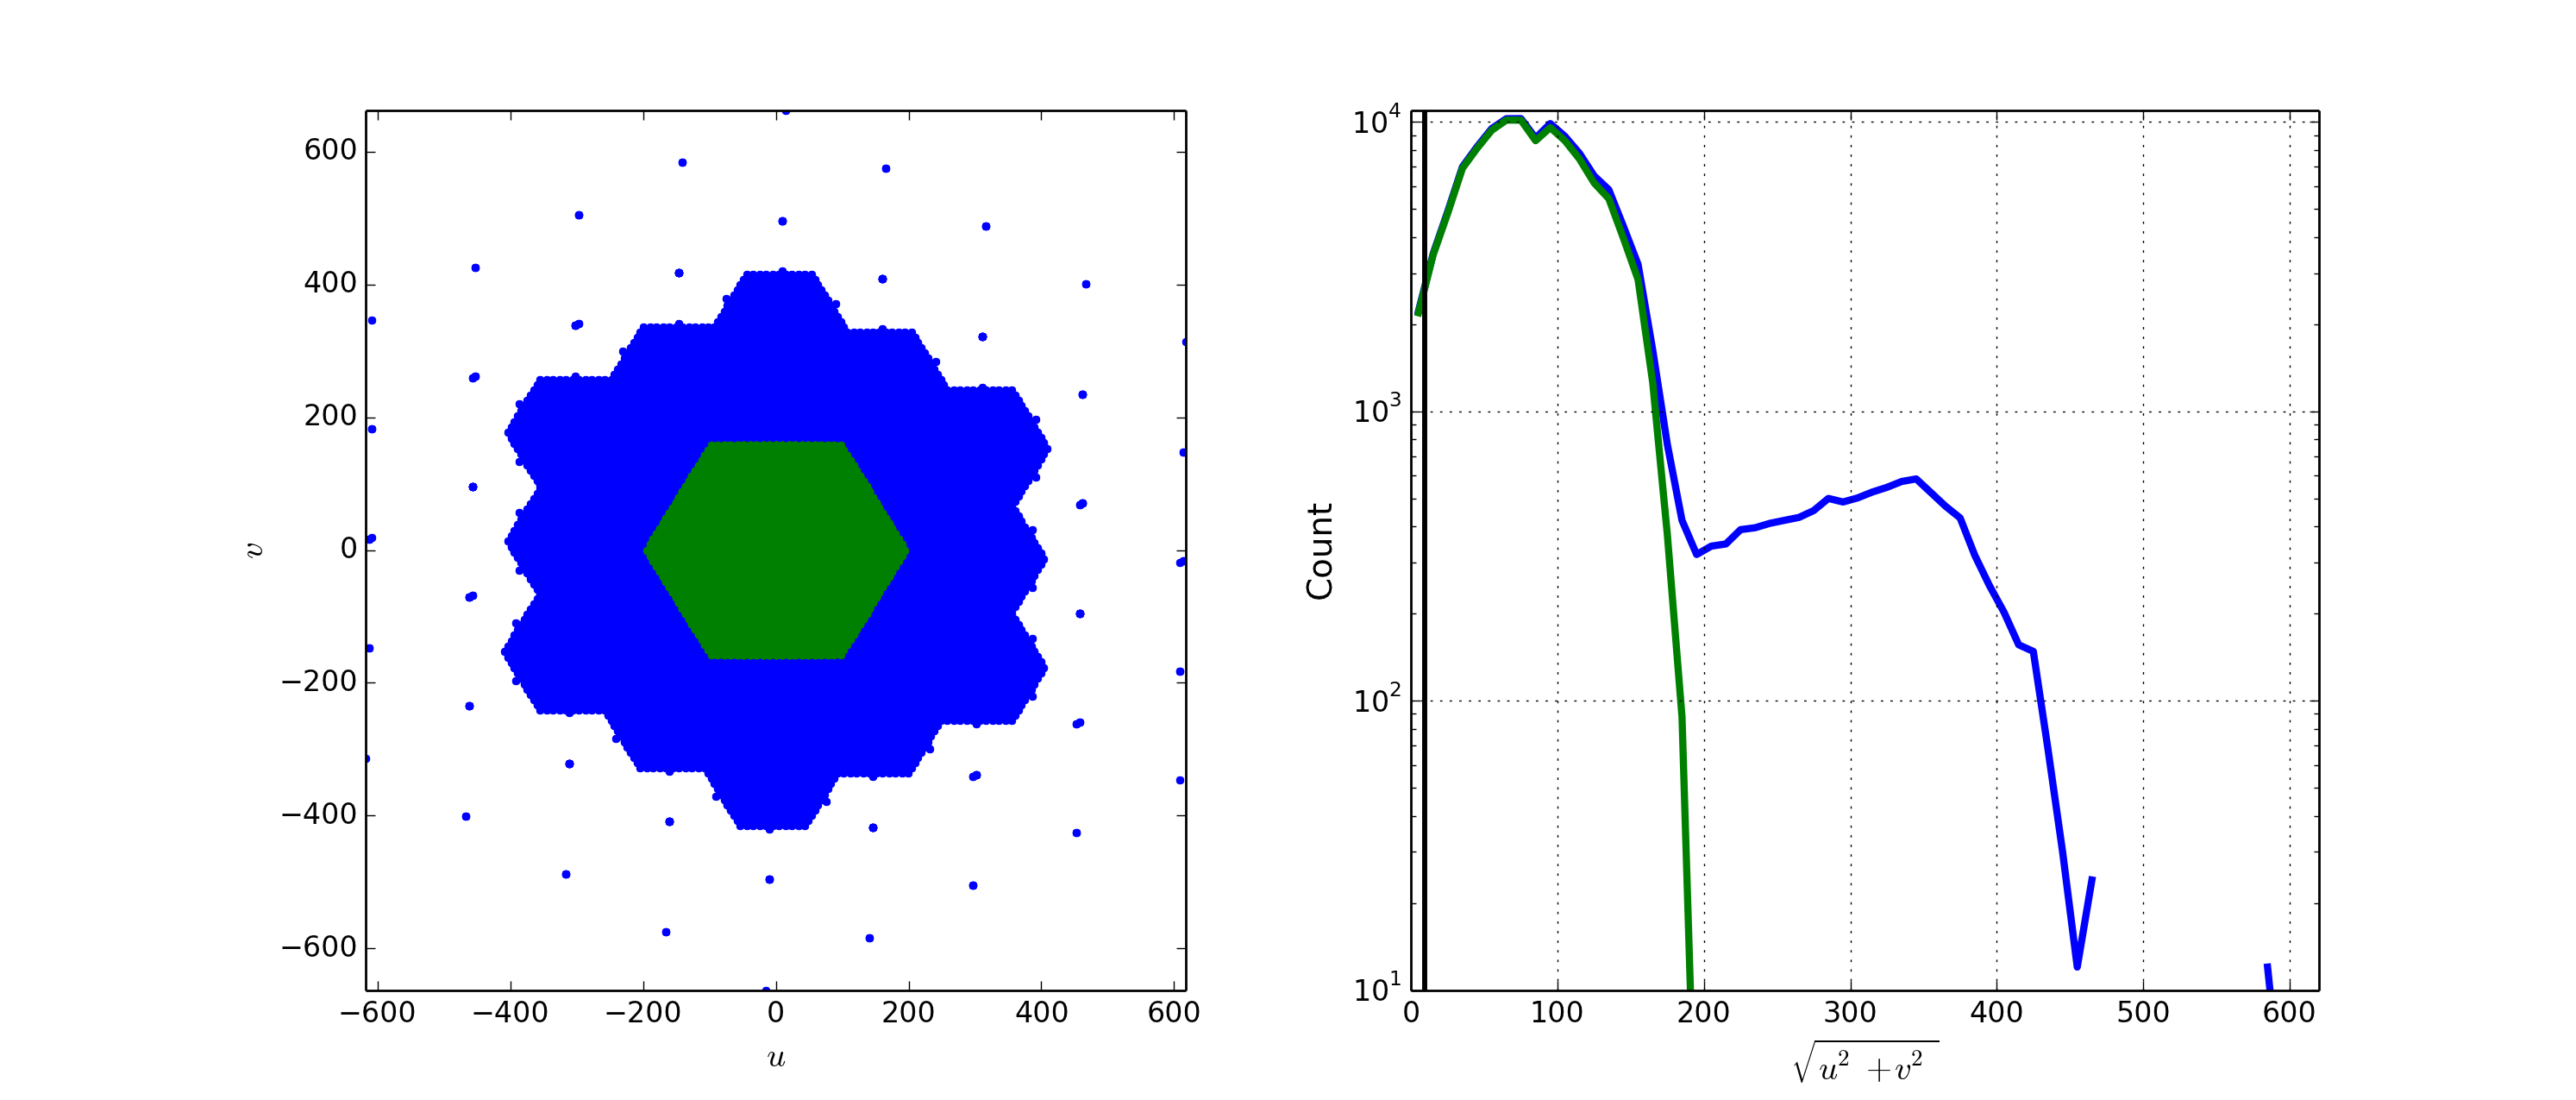
\includegraphics[width=7.5cm]{plots/config.png} 
}
\caption{\small Config
\label{fig:config}}
\end{figure}

\subsection{Calibration}

\section{Conclusion}
A system design meeting the above design principles was presented, which comprises 331 14-meter elements in a compact hexagonal grid and 21 outriggers out to a 1.2km maximum baseline.  HERA uses the demonstrated foreground avoidance technique and should provide a very robust detection of the EOR signal.  Additional work will continue on HERA and other arrays to get the first detection as well as to perfect techniques allowing us to get to the other spatial scales and image the EOR.  Figure \ref{fig:eorsense} compares the sensitivity of existing arrays (left of the thick vertical line) using the different techniques, along with future HERA and SKA arrays.  HERA has the strong potential to get a robust detection in the near-term and characterize the EOR and signal processing to feed into the SKA to get a more complete picture of this period in the life of our early Universe.

\begin{figure}[t]
\centerline{
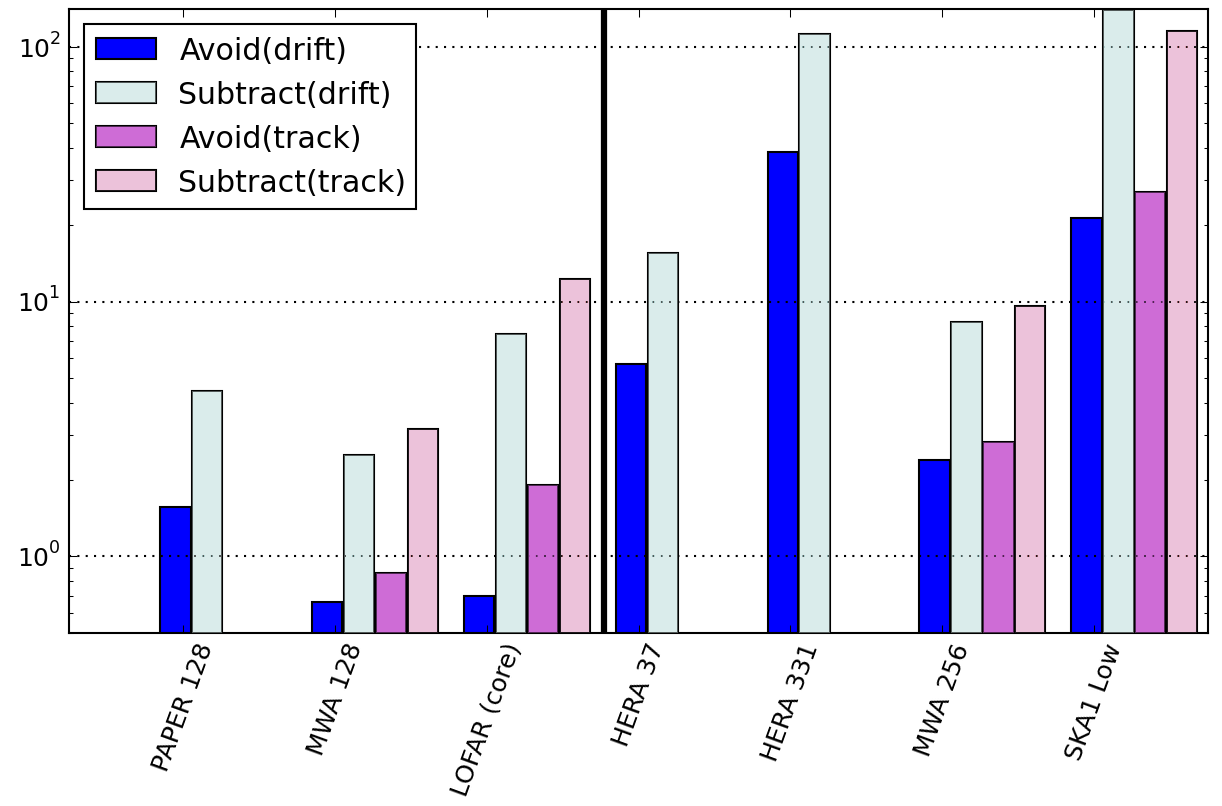
\includegraphics[width=7.5cm]{plots/eorsens.png} 
}
\caption{\small Sensitivity calculations for present and future arrays  (separated by the vertical thick black line) investigating the EOR.
The arrays are mentioned in Sec. \ref{sec:intro}.  The four bars per array refer to different observing and analysis techniques.  The "avoidance" 
methods are largely demonstrated while the "subtraction" ones are still under development.  Note that PAPER/HERA do not track.
\label{fig:eorsense}}
\end{figure}
\section*{Acknowledgments}
This material is based upon work supported by the National Science Foundation Graduate Research Fellowship under Grant No. 1440343.
\bibliographystyle{plain}
\bibliography{mybibdesk}

\end{document}
